\documentclass[border=3pt]{standalone}
\usepackage[svgnames]{xcolor}
\usepackage{tikz}
\usetikzlibrary{positioning}
\usepackage{amsfonts}
\usepackage{pxfonts}

\newcommand{\N}{\ensuremath{\mathbb{N}} }% set of natural numbers

\newcommand{\e}{\mathrm{e}}% exponential number

\newcommand{\definitions}{%
  % color of set of Natural numbers
  \colorlet{colN}{OrangeRed!60}
  % color of set of Integers
  \colorlet{colN0}{OrangeRed!50!Orange!60}
  % color of set of Rational numbers

  % center coordinate of Natural numbers
  \coordinate (oN) at (0.0, 0.0);
  % center coordinate of Integers
  \coordinate (oN0) at (0.25, 0.25);
  % center coordinate of Rational numbers

  % set of Natural numbers
  \def\setN{(oN) ellipse (2.5 and 1.0)}
  % set of Integers
  \def\setZ{(oN0) ellipse (3 and 1.5)}
  % set of Rational numbers
}

\begin{document}
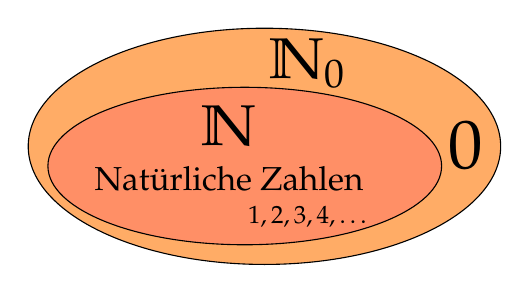
\begin{tikzpicture}
  
  % define colors and sets
  \definitions

  % fill sets in reverse order of size
  \filldraw[fill=colN0]\setZ;
  \filldraw[fill=colN]\setN;

  % add set label for each set
  \node[font=\huge] (N) at (-.2, 0.5) {\N};
  \node[font=\huge] (N0) at (0.8, 1.3) {$\N_0$};

  % add name label for each set
  \node[font=\large] [below=0ex of N] {Natürliche Zahlen};
  \node[font=\large] [below=0ex of N0] {};

  % add number examples for each set
  \node[font=\small] [below right=3ex and -1em of N] {$1,2,3,4,\ldots$};
  \node[font=\small] [below right=1ex and 3em of N0] {\Huge $0$};

\end{tikzpicture}
\end{document}
